\documentclass[a4paper, 12pt]{article} % тип документа

%%%Библиотеки
    %\usepackage[warn]{mathtext}	
    \usepackage[T2A]{fontenc}   %Кодировка
    \usepackage[utf8]{inputenc} %Кодировка исходного текста
    \usepackage[english, russian]{babel} %Локализация и переносы
    \usepackage{caption}
    \usepackage{listings}
    \usepackage{amsmath, amsfonts, amssymb, amsthm, mathtools}
    \usepackage[warn]{mathtext}
    \usepackage[mathscr]{eucal}
    \usepackage{wasysym}
    \usepackage{graphicx} %Вставка картинок правильная
    \usepackage{pgfplots}
    \usepackage{indentfirst}
    \usepackage{float}    %Плавающие картинки
    \usepackage{wrapfig}  %Обтекание фигур (таблиц, картинок и прочего)
    \usepackage{fancyhdr} %Загрузим пакет
    \usepackage{lscape}
    \usepackage{xcolor}
    \usepackage[normalem]{ulem}
    
    \usepackage{titlesec}
    \titlelabel{\thetitle.\quad}

    \usepackage{hyperref}

%%%Конец библиотек

%%%Настройка ссылок
    \hypersetup
    {
        colorlinks = true,
        linkcolor  = blue,
        filecolor  = magenta,
        urlcolor   = blue
    }
%%%Конец настройки ссылок


%%%Настройка колонтитулы
    \pagestyle{fancy}
    \fancyhead{}
    \fancyhead[L]{2.4.1}
    \fancyhead[R]{Глаз Роман, группа Б01-007}
    \fancyfoot[C]{\thepage}
%%%конец настройки колонтитулы



\begin{document}
                        %%%%Начало документа%%%%


%%%Начало титульника
\begin{titlepage}

    \newpage
    \begin{center}
        \normalsize Московский физико-технический институт \\(госудраственный университет)
    \end{center}

    \vspace{6em}

    \begin{center}
        \Large Лабораторная работа по общему курсу физики\\Термодинамика и молекулярная физика
    \end{center}

    \vspace{1em}

    \begin{center}
        \Large \textbf{2.4.1. Определение теплоты испарения жидкости }
    \end{center}

    \vspace{2em}

    \begin{center}
        \large Глаз Роман Сергеевич\\
        Группа Б01-007
    \end{center}

    \vspace{\fill}

    \begin{center}
        Долгопрудный \\2021
    \end{center}
    
\end{titlepage}
%%%Конец Титульника



%%%Настройка оглавления и нумерации страниц
    \thispagestyle{empty}
    \newpage
    \tableofcontents
    \newpage
    \setcounter{page}{1}
%%%Настройка оглавления и нумерации страниц


                    %%%%%%Начало работы с текстом%%%%%%

\textbf{Цель работы:} измерение давления насыщенного пара жидкости при разной температуре; вычисление по полученным данным теплоты испарения с помощью уравнения Клапейрона–Клаузиуса.\\

\textbf{Используемое оборудование:} термостат; герметический сосуд, заполненный исследуемой жидкостью; отсчетный микроскоп.

\section{Теоретическое введение}

Теплоту парообразования жидкостей можно измерить непосредственно при помощи калориметра. Такой метод, однако, не позволяет получить точных результатов из-за неконтролируемых потерь тепла, которые трудно сделать малыми. В настоящей работе для определения теплоты испарения применен
косвенный метод, основанный на формуле Клапейрона–Клаузиуса: 

\begin{equation}
    \frac{dP}
{dT} = \frac{L}{T(V_2 - V_1)}
\end{equation}

Здесь $P$ — давление насыщенного пара жидкости при температуре $T$, $T$ — абсолютная температура жидкости и пара, $L$ — теплота испарения жидкости, $V2$ — объем пара, $V_1$ — объем жидкости. Найдя из опыта $\frac{dP}{dT},\; T,\; V_2$ и $V_1$, можно определить $L$ путем расчета. Величины $L, \;V_2$ и $V_1$ в формуле $(1)$ должны относиться к одному и тому же количеству вещества; мы будем относить их к одному молю.
В нашем приборе измерения производятся при давлениях ниже атмосферного. В этом случае задача существенно упрощается.

С помощью уравнения Ван-дер-Ваальса можно получить зависимость $P(T)$, с помощью которой определить искомую величину:

\begin{equation}
    \left(P+\frac{a}{V^2}\right)(V-b) = RT
\end{equation}

В таблице ниже приведены все значения параметров различных жидкостей уранения Ван-дер-Ваальса в условиях данного опыта.

\begin{figure}[h]
    \center{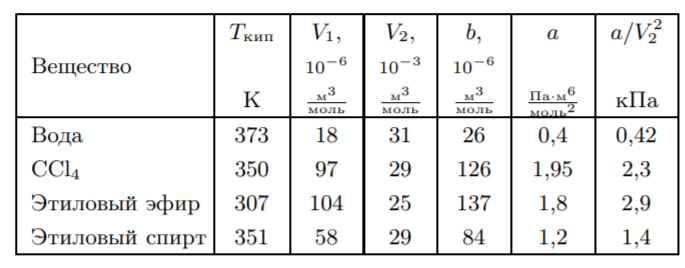
\includegraphics[scale = 1]{lab_2_4_1_tablica}}
\end{figure}

Откуда видно, что $\frac{V_1}{V_2} < 0,005$, a $\frac{a}{PV^2}<0,03$, ошибка метода измерений равна $4\%$, тогда записав уравнение Клапейрона-Менделеева для насыщенного пара, получим:
$V=\frac{RT}{P}\;.$
Пренебрегая $V_1$ (который не превосходит $0,5\%$ от $V_2$), запишем:

\begin{equation}
    L=\frac{RT^2}{P} \frac{dP}{dT} = -R\frac{d(lnP)}{d(1/T)}
\end{equation}

Эта формула является окончательной.

\section{Эксперементальная установка}

Схема установки изображена на рисунке $1$. Наполненный водой резервуар $1$ играет роль термостата. Нагревание термостата производится спиралью $2$, подогреваемой электрическим током. Для охлаждения воды в термостате через змеевик $3$ пропускается водопроводная вода. Вода в термостате перемешивается воздухом,
поступающим через трубку $4$. Температура воды измеряется термометром $5$. В термостат погружен запаянный прибор $6$ с исследуемой жидкостью. Над ней находится насыщенный пар (перед заполнением прибора воздух из него был откачан).
Давление насыщенного пара определяется по ртутному манометру,соединенному с исследуемым объемом. Отсчет показаний манометра производится при помощи микроскопа.

\begin{figure}[h]
    \center{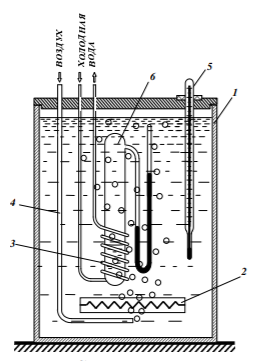
\includegraphics[scale = 1.5]{lab_2_4_1_ust}}
    \caption{Схема установки для определения теплоты испарения}
\end{figure}

\section{Снятие данных}

Измерим разность уровней в ртутном $U$-образном манометре с помощью микроскопа и температуру по термометру. $H$ - высота высокого колена, $h$ - низкого. При этом будем настраивать микроскоп так, чтобы каждый раз основание мениска было у метки прибора (в дальнейшем считаем, что высота мениска не меняется, не смотря на то что поверхностное натяжение ртути на самом деле зависит от температуры и высота немного должна меняться). Результаты представлены в таблицах $1$ и $2$. Под $P_0$ подразумевается давление $1$ мм рт.ст.

Приведём формулы для рассчётов погрешностей.
Поскольку давление напрямую зависит от разности уровней ртути (пренебрегаем давлением насыщенных паров ртути, так как при комнатной температуре оно приблизительно равно $0,24$ Па, а так же изменением уровня столба воды, так как он слишком мал), то для погрешности давления $P$ воспользуемся следующей формулой: 

\begin{equation}
    \sigma_P = P_{\text{aтм}} \cdot \frac{\sigma_{H-h}}{H_0}
\end{equation}

где под $H_0$ подразумевается $760$ мм, а под $P_{\text{атм}} = 101325 \; \text{Па}$ - нормальное атмосферное давленине. В качестве $\sigma_{H-h}$ будем брать $2$ мм, поскольку точность измерения каждого из уровня $0,1$ мм, а так же мы будем учитывать, что $U$-образный манометр в нашей установке был не вертикален, а немного наклонён.

\begin{equation}
    \sigma_{\ln{\frac{P}{P_0}}} = \frac{\sigma_P}{P}
\end{equation}

Погрешность определения температуры возьмём учитывая точность прибора и тот факт, что во время измерений уровней температура могла немного изменяться: $\sigma_{T} = 0,2 \; K$.

Соответсвенно

\begin{equation}
    \sigma_{\frac{1}{T}} = \frac{\sigma_T}{T^2}
\end{equation}

Снимем все точки данных, проведя сам эксперимент (см. таблицы).

\begin{center}
\begin{table}[h]
        \caption{При нагреве}
\begin{tabular}{|c|c|c|c|c|c|c|c|}
    \hline 
    $h ,\; {\text{см}}$  & 7,73 & 7,71 & 7,66 & 7,60 & 7,55 & 7,465 & 7,38 \\ 
    \hline 
    $H, \; \text{см}$ & 9,91  & 9,94  & 9,97 & 10,05 & 10,13 & 10,18 & 10,24  \\ 
    \hline 
    $P \cdot 10^2,\; \text{Па}$ & 28,99  & 29,53 & 30,72 & 32,59 & 34,31 & 36,17  & 38,04\\ 
    \hline 
    $\sigma_{P}, \text{Па}$  & \multicolumn{7}{|c|}{266}  \\
    \hline 
    $\ln(P)$  & 7,970 & 7,990 & 8,031 & 8,090 & 8,141 & 8,193 & 8,244 \\ 
    \hline 
    $\sigma_{\ln(P)} \cdot 10^{-2}$ & 9,207 & 9,007 & 8,659 & 8,162 & 7,753 & 7,354 & 6,992 \\ 
    \hline
    $T,\; K$ & 291,81 & 292,84 & 294,00 & 295,14 & 296,60 & 298,14 & 299,15 \\
    \hline
    $\sigma_{T},\; {K}$ &\multicolumn{7}{|c|}{0,2} \\
    \hline 
    $\frac{10^3}{T},{K}^{-1}$ & 3.427  & 3,414 & 3,401 & 3,388 & 3,371 & 3,354 & 3,343\\ 
    \hline
    $\sigma_{\frac{1}{T}} \cdot 10^{-6},\; {K}^{-1}$ & 2.292 & 2.263  & 2.242 & 2.223 &  2.206 & 2.183 & 2.154  \\
    \hline
\end{tabular}

\begin{tabular}{|c|c|c|c|c|c|c|c|}
    \hline 
    $h ,\; {\text{см}}$  & 7,28 & 7,10 & 6,75 & 6,63 & 6,46  & 6,39 & 6,27 \\ 
    \hline 
    $H, \; \text{см}$ & 10,39  & 10,61  & 10,92 & 11,09 & 11,22 & 11,34 & 11,47   \\ 
    \hline 
    $P \cdot 10^2,\; \text{Па}$ & 41,36  & 46,68 & 55,46 & 59,32 & 63,31 & 65,84  & 69,16\\ 
    \hline 
    $\sigma_{P}, \text{Па}$  & \multicolumn{7}{|c|}{266}  \\
    \hline 
    $\ln(P)$  & 8,328 & 8,449 & 8,620 & 8,688 & 8,753 & 8,792 & 8,842 \\ 
    \hline 
    $\sigma_{\ln(P)} \cdot 10^{-2}$ & 6,431 & 5,698 & 4,796 & 4,484 & 4,201 & 4,040 & 3,846 \\ 
    \hline
    $T,\; K$ & 301,11 & 303,35 & 306,75 & 308,25 & 309,53 & 310,55 & 311,73 \\
    \hline
    $\sigma_{T},\; {K}$ &\multicolumn{7}{|c|}{0,2} \\
    \hline 
    $\frac{10^3}{T},{K}^{-1}$ & 3,321 & 3,297 & 3,260 & 3,244 & 3,231 & 3,220 & 3,208\\ 
    \hline
    $\sigma_{\frac{1}{T}} \cdot 10^{-6},\; {K}^{-1}$ & 2.292 & 2.263  & 2.242 & 2.223 &  2.206 & 2.183 & 2.154  \\
    \hline
\end{tabular}

\begin{tabular}{|c|c|c|c|c|c|c|c|}
    \hline 
    $h ,\; {\text{см}}$  & 6,07 & 5,90 & 5,71 & 5,44 & 5,26  & 4,79 & 4,55 \\ 
    \hline 
    $H, \; \text{см}$ & 11,72 & 11,88  & 12,08 & 12,32 & 12,56 &  13,03 & 13,32 \\ 
    \hline 
    $P \cdot 10^2,\; \text{Па}$ & 75,15  & 79,67 & 84,72 & 91,50 & 97,09 & 109,59  & 116,64\\ 
    \hline 
    $\sigma_{P}, \text{Па}$  & \multicolumn{7}{|c|}{266}  \\
    \hline 
    $\ln(P)$  & 8,925 & 8,983 & 9,044 & 9,122 & 9,181 & 9,302 & 9,364 \\ 
    \hline 
    $\sigma_{\ln(P)} \cdot 10^{-2}$ & 3,539 & 3,339 & 3,140 & 2,907 & 2,739 & 2,427 & 2,280 \\ 
    \hline
    $T,\; K$ & 313,15 & 314,37 & 315,75 & 317,05 & 318,38 & 320,63 & 321,90 \\
    \hline
    $\sigma_{T},\; {K}$ &\multicolumn{7}{|c|}{0,2} \\
    \hline 
    $\frac{10^3}{T},{K}^{-1}$ & 3,193 & 3,180 & 3,167 & 3,154 & 3,141 & 3,119 & 3,107\\ 
    \hline
    $\sigma_{\frac{1}{T}} \cdot 10^{-6},\; {K}^{-1}$ & 2.292 & 2.263  & 2.242 & 2.223 &  2.206 & 2.183 & 2.154  \\
    \hline
\end{tabular}
\end{table}

\begin{table}[h]
    \caption{При охлаждении}
\begin{tabular}{|c|c|c|c|c|c|c|c|c|}
    \hline 
    $h ,\; {см}$ &  4,79 & 5,07 & 5,42 & 5,57 & 5,95 & 6,12 & 6,33  \\ 
    \hline 
    $H, \; {см}$ &  13,20  & 12,72  & 12,42 & 12,04 & 11,84 & 11,62 & 11,46 \\ 
    \hline 
    $P \cdot 10^2,\; \text{Па}$ &  111,85  & 101,75 & 93,10 & 86,05 & 78,34 & 73,15 & 68,23 \\ 
    \hline 
    $\sigma_{P}, \text{Па}$  & \multicolumn{7}{|c|}{266}  \\
    \hline
    $\ln(P)$ & 9,322  & 9,228 & 9,139 & 9,060 & 8,996 & 8,898 & 8,828\\ 
    \hline 
    $\sigma_{\ln(P)} \cdot 10^{-2}$ & 2,378 & 2,614 & 2,857 & 3,093 & 3,395 & 3,630 & 3,899\\ 
    \hline
    $T , \; {K}$ & 320,15  & 318,15 & 316,05 & 314,15 & 312,45 & 311,15 & 309,65 \\ 
    \hline
    $\sigma_{T},\; {K}$ & \multicolumn{7}{|c|}{0,2} \\
    \hline
    $\frac{10^3}{T},{K}^{-1}$ & 3,124 & 3,143 & 3,164 & 3,183 & 3,200 & 3,214 & 3,230\\ 
    \hline 
    $\sigma_{\frac{1}{T}} \cdot 10^{-6}, \; {K}^{-1}$   & 2.215  & 2.191 & 2.177 & 2.169 & 2.134 & 2.123 &  2.107 \\ 
    \hline
\end{tabular} 

\begin{tabular}{|c|c|c|c|c|c|c|c|c|}
    \hline 
    $h ,\; {см}$ &  6,49 & 6,59 & 6,66 & 6,79 & 6,86 & 6,97 & 7,04  \\ 
    \hline 
    $H, \; {см}$ &  11,23  & 11,14  & 11,01 & 10,93 & 10,80 & 10,73 & 10,64 \\ 
    \hline 
    $P \cdot 10^2,\; \text{Па}$ &  63,04  & 60,52 & 57,85 & 55,06 & 52,40 & 50,00 & 47,88 \\ 
    \hline 
    $\sigma_{P}, \text{Па}$  & \multicolumn{7}{|c|}{266}  \\
    \hline
    $\ln(P)$ & 8,749 & 8,708 & 8,663 & 8,614 & 8,564 & 8,517 & 8,474\\ 
    \hline 
    $\sigma_{\ln(P)} \cdot 10^{-2}$ & 4,219 & 4,395 & 4,598 & 4,831 & 5,076 & 5,320 & 5,555\\ 
    \hline
    $T , \; {K}$ & 307,95  & 307,15 & 306,15 & 305,15 & 304,15 & 303,15 & 302,15 \\ 
    \hline
    $\sigma_{T},\; {K}$ & \multicolumn{7}{|c|}{0,2} \\
    \hline
    $\frac{10^3}{T},{K}^{-1}$ & 3,247 & 3,256 & 3,266 & 3,277 & 3,288& 3.299 & 3,309\\ 
    \hline 
    $\sigma_{\frac{1}{T}} \cdot 10^{-6}, \; {K}^{-1}$   & 2.215  & 2.191 & 2.177 & 2.169 & 2.134 & 2.123 &  2.107 \\ 
    \hline
\end{tabular} 

\begin{tabular}{|c|c|c|c|c|c|c|c|c|}
    \hline 
    $h ,\; {см}$ &  7,13 & 7,19 & 7,26 & 7,34 & 7,41 & 7,46 & 7,53  \\ 
    \hline 
    $H, \; {см}$ &  10,56  & 10,45  & 10,39 & 10,32 & 10,24 & 10,17 & 10,12  \\ 
    \hline 
    $P \cdot 10^2,\; \text{Па}$ & 45,62 & 43,42 & 41,63 & 39,63 & 37,51 & 36,04 & 34,45 \\ 
    \hline 
    $\sigma_{P}, \text{Па}$  & \multicolumn{7}{|c|}{266}  \\
    \hline
    $\ln(P)$ & 8,426  & 8,376 & 8,333 & 8,285 & 8,230 & 8,190 & 8,144\\ 
    \hline 
    $\sigma_{\ln(P)} \cdot 10^{-2}$ & 5,830 & 6,126 & 6,389 & 6,712 & 7,091 & 7,380 & 7,721\\ 
    \hline
    $T , \; {K}$ & 301,15  & 300,15 & 299,15 & 298,15 & 297,15 & 296,15 & 295,15 \\ 
    \hline
    $\sigma_{T},\; {K}$ & \multicolumn{7}{|c|}{0,2} \\
    \hline
    $\frac{10^3}{T},{K}^{-1}$ & 3,320 & 3,332 & 3,343 & 3,354 & 3,365 & 3,376 & 3,387\\ 
    \hline 
    $\sigma_{\frac{1}{T}} \cdot 10^{-6}, \; {K}^{-1}$   & 2.215  & 2.191 & 2.177 & 2.169 & 2.134 & 2.123 &  2.107 \\ 
    \hline
\end{tabular} 
\end{table}
\end{center}

\section{Аппроксимация полученных данных}

Как было сказано в теоретическом введении, согласно формуле $(3)$, график зависимости $ln(P)\left( \frac{1}{T}\right)$ -- убывающая прямая. Учитывая, что известны погрешности $\sigma_{ln(P)} \gg \sigma_{\frac{1}{T}}$, определим характеристики прямой графика с помощью метода Пирсона (хи-квадрат) по следующим формулам:

\begin{equation}
    L = - \frac{\langle \frac{ln(P)}{T} \rangle ' - \langle ln(P) \rangle ' \langle \frac{1}{T} \rangle ' }{\langle \frac{1}{T^2} \rangle ' - \left( \langle \frac{1}{T} \rangle ' \right)^2}
\end{equation}

\begin{equation}
    C =  \langle ln(P) \rangle ' + L  \langle \frac{1}{T} \rangle '
\end{equation}

\begin{equation}
    ln(P) = -\frac{L}{T} + C
\end{equation}

По этим формулам получим следующие значения при нагревании:

\begin{equation}
    L_{\text{н}} = 4,431 \cdot 10^4 \; \frac{\text{Дж}}{\text{К}}, \Delta L_{\text{н}} = 9,867 \cdot 10^2 \; \frac{\text{Дж}}{\text{К}}\; 
\end{equation}

\begin{equation}
    C_{\text{н}} = 23,079, \; \Delta C_{\text{н}} = 0,445
\end{equation}

\begin{equation}
    L_{\text{охл}} = 4,508 \cdot 10^4 \; \frac{\text{Дж}}{\text{К}}, \Delta L_{\text{охл}} = 9,654 \cdot 10^2 \; \frac{\text{Дж}}{\text{К}}\; 
\end{equation}

\begin{equation}
    C_{\text{охл}} = 23,399, \; \Delta C_{\text{охл}} = 0,427
\end{equation}

Так как $C_{\text{охл}} -C_{\text{н}} = 0,320 < \Delta C \cong 0,43 $ (в качестве оценки), то различить две отдельные прямые для нагревания и охлаждения невозможно.

Заметим, что значение удельной теплоты парообразования воды при нагревании сходится с табличным значением больше, чем при охлаждении ($L = 4,04 \cdot 10^4 \; \frac{\text{Дж}}{\text{К}}$)

Теперь нужно учесть погрешности, вызванные методическими приближениями. 

Первое, что нужно учесть -- давление насыщенного пара ртути, которым мы пренебрегли при расчёте погрешностей ввиду его малости по сравнению с атмосферным давлением:

\begin{equation}
    \frac{\Delta L_P  }{L} = \frac{P_s}{P} = \frac{0,26}{3 \cdot 10^3} = 8,667 \cdot 10^{-5}
\end{equation}

Эта формула следует напрямую из уравнения Клапейрона-Клаузиуса.

Теперь посчитаем относительную погрешность:

\begin{equation}
    \frac{\Delta L_{\text{охл}}}{L_{\text{охл}}} = 0,0214
\end{equation}

\begin{equation}
    \frac{\Delta L_{\text{н}}}{L_{\text{н}}} = 0,0223
\end{equation}

Стоить отметить, что погрешности вышли заниженными, так как следует учитывать также следующие факторы, которые измерить тяжело: температура термометра в точности не совпадает с температурой пара из-за неравномерности распределения температуры в термостате, из-за капиллярных эффектов давление насыщенного пара должно быть больше, чем просто разность высот в трубках.

Всё же можно видеть, что полученные значения хорошо соответствуют ранее описанной теории. Для убедительности построим графики $P(T)$ и $ln(P)\left( \frac{1}{T}\right)$.

\begin{figure}
    \begin{center}
        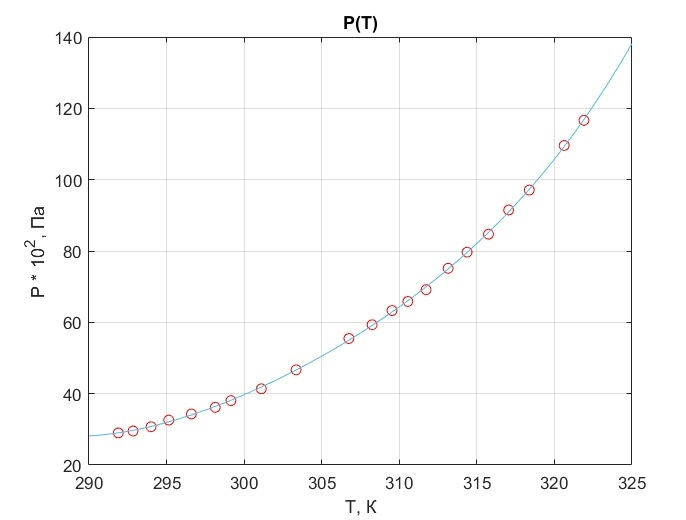
\includegraphics[scale = 0.45]{graph1}
        \caption{$P(T)$ при нагревании}
    \end{center}
\end{figure}

\begin{figure}
    \begin{center}
        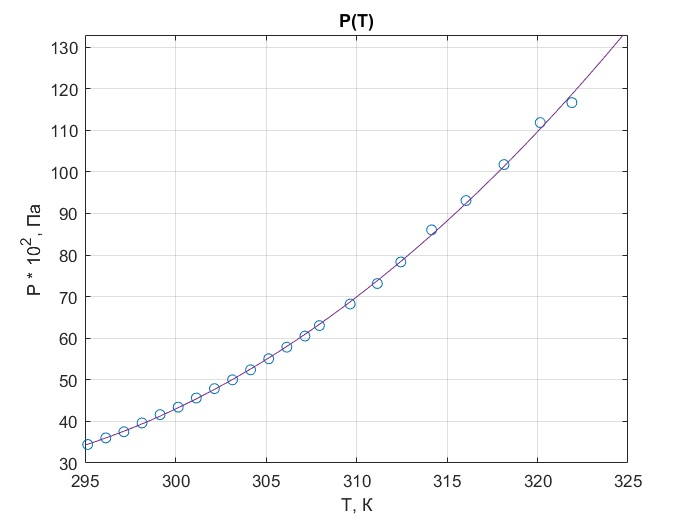
\includegraphics[scale = 0.74]{xgraph1}
        \caption{$P(T)$ при охлаждении}
    \end{center}
\end{figure}

\begin{figure}
    \begin{center}
        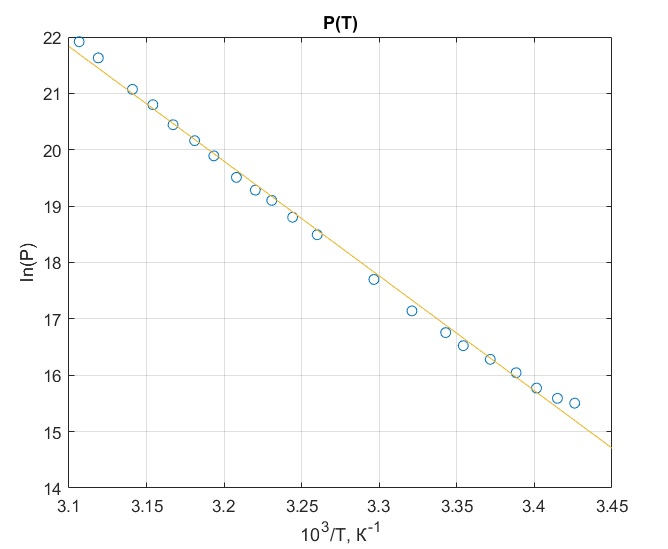
\includegraphics[scale = 0.74]{graph2}
        \caption{$ln(P)(\frac{1}{T})$ при нагревании}
    \end{center}
\end{figure}

\begin{figure}
    \begin{center}
        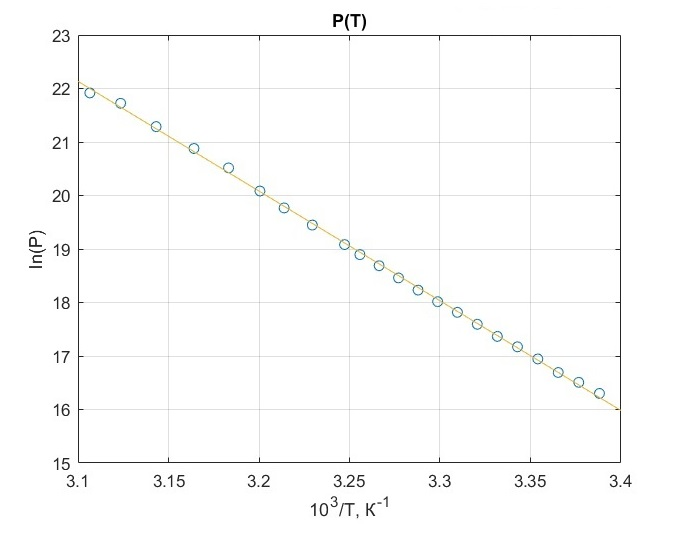
\includegraphics[scale = 0.74]{xgraph2}
        \caption{$ln(P)(\frac{1}{T})$ при охлаждении}
    \end{center}
\end{figure}

Также оценим качество аппроксимации прямой методом хи-квадрат. При нормальном распределении величина $\chi^2 = n - p$, где $n$ -- количество параметров завимости, а $p = 2$, где $n - p$ -- количество линейно независимых параметров в системе уравнений хи-квадрат. В нашем случаем имеем:

\begin{equation}
    \left( \frac{\chi^2}{n - p}\right)_{\text{н}} = \frac{27,453}{19} = 1,445
\end{equation}

\begin{equation}
    \left( \frac{\chi^2}{n - p}\right)_{\text{охл}} = \frac{27,178}{19} = 1,431
\end{equation}

Значения в точности не могут быть равны единице по следующим причинам: во-первых, распределение в данном случае отличается от нормального, во-вторых, погрешность $\frac{1}{T}$ так же стоит брать в учёт, а в методе хи-квадрат в формулах ей пренебрегают.


\section{Заключение}

В работе изучалась зависимость давления насыщенного пара воды от температуры. По полученным данным были найдены коэффициенты удельного испарения воды при нагревании и охлаждении жидкости. Все возникшие параметры были проверены на аппроксимацию и были вычислены все возможные погрешности полученных величин.

\section{Список используемой литературы}

$\bullet$ Гладун А. Д. Лабораторный практикум по общей физике. Термодинамика и молекулярная физика\\

$\bullet$ \href{https://mipt.ru/education/chair/physics/S_II/lab/}{Описание лабораторных работ на кафедре общей физики МФТИ}

\end{document}
